\documentclass[aspectratio=169]{beamer}
\usetheme{metropolis}

\usepackage{roboto}
\usepackage{mathtools}
\usepackage{fixmath}
\usepackage{graphicx}
\usepackage{tikz}
\usepackage{stmaryrd}
\usepackage{listings}
\usepackage{minted}

\graphicspath{ {./images/} }
\setbeamertemplate{navigation symbols}{}

\DeclarePairedDelimiter\Brackets{\llbracket}{\rrbracket}

\title{MIN SET COVER online}
\author{Georg Dorndorf, Louis Milhaud \& Niranjan Nair}
\institute{Université Paris Saclay}
\date{\today}

\begin{document}

    \AtBeginSection[]{
    \begin{frame}
    \vfill
    \centering
    \begin{beamercolorbox}[sep=8pt,center,shadow=true,rounded=true]{title}
        \usebeamerfont{title}\insertsectionhead\par%
    \end{beamercolorbox}
    \vfill
    \end{frame}
    }
    % frame 1
    \begin{frame}
        \titlepage
    \end{frame}

    % frame 2
    \begin{frame}
        \frametitle{Outline}
        \tableofcontents
    \end{frame}

    % frame 3
    \section{Algorithms}
    
    \subsection{Full random algorithm}
    %frame 6
    \begin{frame}[fragile]{Full random algorithm}
    Pseudo-python code for the naive random algorithm:
    \rule{\textwidth}{1pt}
    \scriptsize
    \begin{minted}{python}
        for sigma_i in sequence:
            if sigma_i in cover:
                continue
            else:
                c_i = all_sets_containing_sigma_i(sigma_i, S)
                cover.add(random.choice(c_i))
    \end{minted}
    \rule{\textwidth}{1pt}
    \end{frame}
    
    \subsection{Biggest cover algorithm}
    %frame 7
    \begin{frame}[fragile]{Biggest cover algorithm}
    Pseudo-python code for the biggest cover algorithm:
    \rule{\textwidth}{1pt}
    \scriptsize
    \begin{minted}{python}
        for sigma_i in sequence:
            if sigma_i in cover:
                continue
            else:
                c_i = all_sets_containing_sigma_i(sigma_i, S)
                for c_j_i in c_i:
                    uncovered_size = len(c_j_i) - len(c_j_i.inter(covered_elem))
                    if uncovered_len > max_uncovered_len:
                        choice = c_j_i
                        max_uncovered_size = uncovered_size
    \end{minted}
    \rule{\textwidth}{1pt}
    \end{frame}
    
    \section{Competitivity}
    \begin{frame}{Costs comparison}
        \hspace*{-1.05in}
        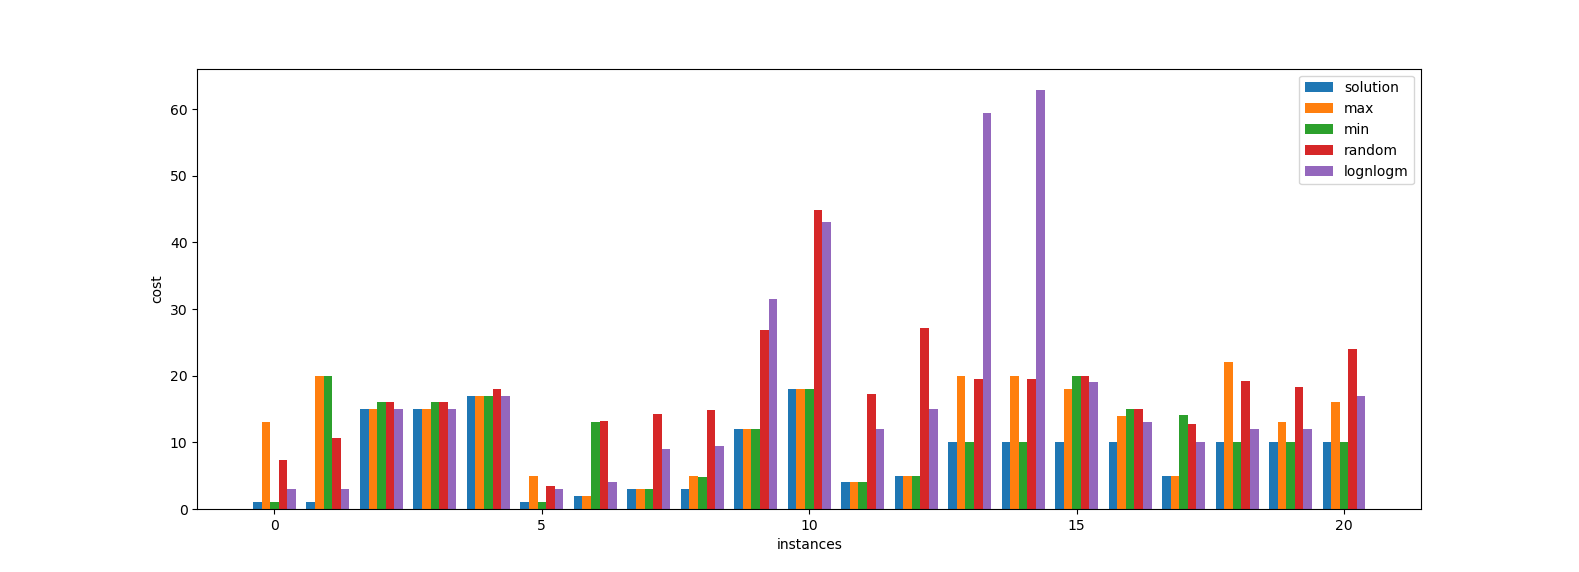
\includegraphics[scale=0.48]{images/costs.png}
    \end{frame}
    \begin{frame}{Competitivity ratios}
        \hspace*{-1in}
        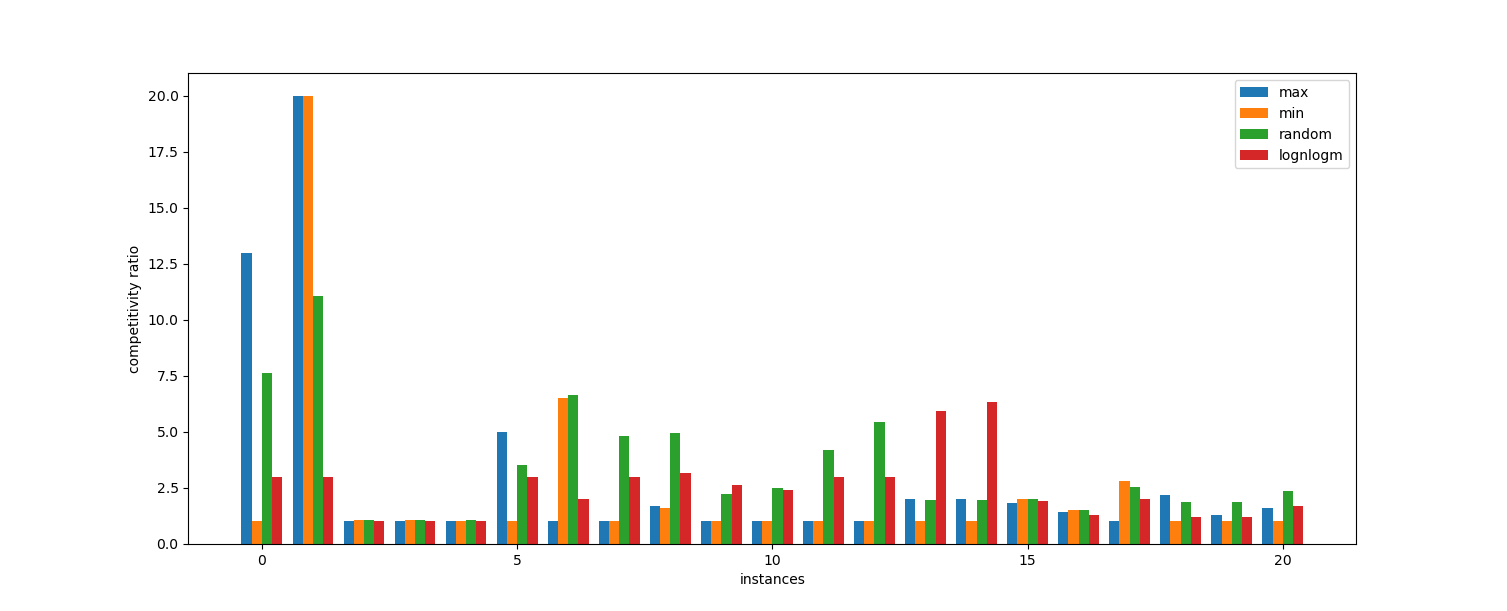
\includegraphics[scale=0.5]{images/competitivity ratio.png}
    \end{frame}

\end{document}